\documentclass[12pt,a4paper]{article}

% Кодування/мови — в такому порядку
\usepackage[utf8]{inputenc}
\usepackage[T2A]{fontenc}
\usepackage[ukrainian]{babel}
\usepackage{cmap}

\usepackage{geometry}
\geometry{left=2cm,right=2cm,top=2cm,bottom=2cm}

\usepackage{graphicx}
\usepackage{array,multirow,booktabs,makecell}
\usepackage{caption}
\renewcommand{\thetable}{\arabic{table}}
\captionsetup[table]{name=Таблиця}

\usepackage{amsmath}
\usepackage{pdflscape}
\usepackage{xcolor}

\newcommand{\g}{\cellcolor{gray!25}} % коротке позначення сірого

% Гіперпосилання — тримай наприкінці пакетів, з unicode
\usepackage[unicode]{hyperref}

\renewcommand\cellalign{tc}
\renewcommand\theadalign{cc}
\newcommand{\addh}{\rule{0pt}{3.8ex}} % ДОДАТКОВА ВИСОТА РЯДКА (лише де потрібно)
\renewcommand{\arraystretch}{1.25}

\begin{document}

    \begin{titlepage}

        % Картинка шапки (по центру, з відступом від верху)
        \begin{center}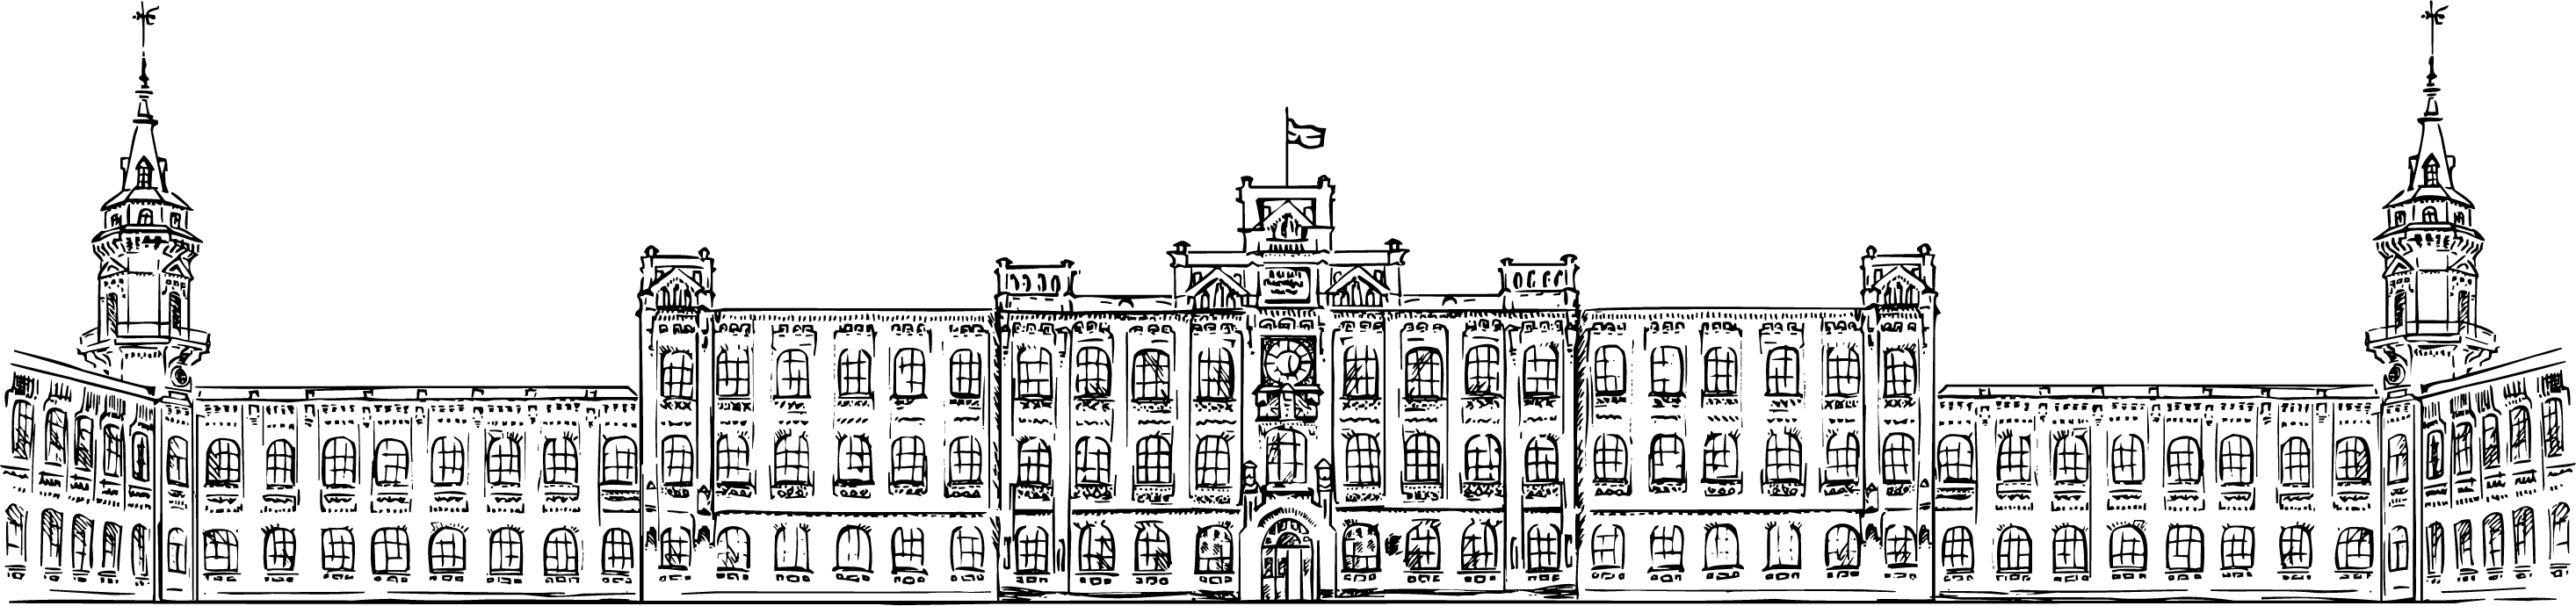
\includegraphics[width=0.7\textwidth]{../../../TITLES/letterhead.png}\end{center}

        \begin{center}
            \large Національний технічний університет України\\
            «Київський політехнічний інститут імені Ігоря Сікорського»\\[1em]
            Факультет інформатики та обчислювальної техніки\\
            Кафедра обчислювальної техніки
        \end{center}

        \vfill

        \begin{center}
            \textbf{\LARGE Теорія електричних кіл та сигналів}\\[2em]
            \textbf{\Large Лабораторна робота №8}\\[0.5em]
            «Дослідження перехідних процесів у електричних колах з послідовним з'єднанням резистивно-індуктивно-ємнісних (RLC) елементів»
        \end{center}

        \vfill

        \begin{flushright}
            Виконав: студент 2 курсу ФІОТ, гр. ІО-41\\
            \textit{Давидчук A.~M.}\\[1em]
            Перевірив: \textit{Лободзинський В.~Ю.}
        \end{flushright}

        \vfill

        \begin{center}Київ --- 2025\end{center}

    \end{titlepage}

    \noindent
    \textbf{\underline{Тема:}} «Дослідження перехідних процесів у електричних колах з послідовним з'єднанням резистивно-індуктивно-ємнісних (RLC) елементів».

    \vspace{1em}

    \noindent
    \textbf{\underline{Мета:}} Дослідження перехідних процесів в електричних колах постійного струму
    при послідовному з’єднанні: резистивно-індуктивно-ємнісних (RLC)
    елементів.

    \begin{center} \textbf{\Large Практична частина} \end{center}

    Усі розрахунки було проведено за допомогою мови програмування Python (вихідний код додано разом із звітом).

    \begin{center} \textbf{\large Завдання №1 (офлайн частина)} \end{center}

    Загальна структурна схема електричного кола:

    \begin{figure}[h!]

        \renewcommand{\thefigure}{\arabic{figure}} % робимо "3.1", "3.2" і т.д.

        \centering
        \includegraphics[width=0.4\textwidth]{sc.pdf}
        \caption{Структурна схема електричного кола}

    \end{figure}

    Звідси параметри елементів (для I бригади):

    \[
    R_4 = 50 \text{ Ом} \quad L_4 = 60 \text{ мГн} \quad C_4 = 3 \text{ мкФ} \quad R_0 = 50 \text{ Ом}
    \]

    Виміряний опір котушки $R_{\text{к}}$ за допомогою Омметра: $R_{\text{к}} = 35{,}5$ Ом.

    Змальовані криві зміни $u_R(t)$, $u_L(t)$, $u_C(t)$ у масштабі з екрану осцилографа (коливальний процес):

    \begin{figure}[h!]

        \renewcommand{\thefigure}{\arabic{figure}} % робимо "3.1", "3.2" і т.д.

        \centering
        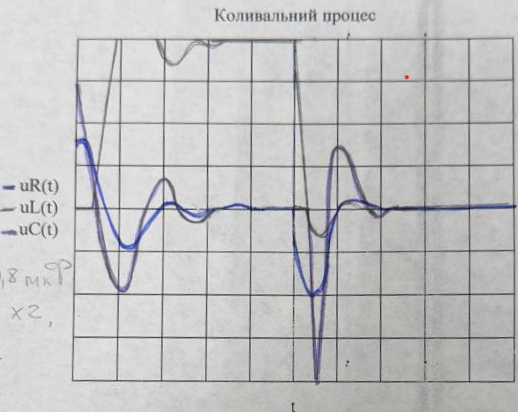
\includegraphics[width=0.5\textwidth]{vgg.png}
        \caption{\centering Осцилограми напруг на елементах RLC-контуру: $u_R(t)$, $u_L(t)$, $u_C(t)$ під час коливального процесу.}

    \end{figure}

    І підібрана ємність $C$ при якій частота коливань $\omega'$ зарядного струму подвоїться (при цьому період коливань зменшиться вдвічі): $C_2 = C = 0{,}8$ мкФ.

    Розрахуємо критичний опір всього контуру $R_{\text{кр}}$ при якому відбувається перехід до критичного режиму:

    \[
    R_{\text{кр}} = 2 \sqrt{\frac{L_4}{C_4}}  = 2 \sqrt{\frac{60 \cdot 10^{-3}}{3 \cdot 10^{-6}}} \approx 282{,}84 \text{ Ом}
    \]

    Тепер експериментально перевіримо розрахунок опору переходу до критичного режиму, шляхом зміни опору $R_4$ в колі, тим самим змінюючи загальний опір всього контуру.
    Опір $R_4'$ при якому коливальний процес переходить у аперіодичний (критичний) дорівнює:

    \[
    R_4 = 247 \text{ Ом}
    \]

    Враховуючи, що $R = R_{\text{к}} + R_4'$, маємо, що

    \[
    R_{\text{кр/експ.}} = R_{\text{к}} + R_4' = 35{,}5 + 247 \approx 282{,}5 \text{ Ом}
    \]

    Як бачимо, різниця між розрахунковим та експериментальним значенням критичного опору є дуже малою.

    Змальовані криві зміни $u_R(t)$, $u_L(t)$, $u_C(t)$ у масштабі з екрану осцилографа (критичний режим):

    \begin{figure}[h!]

        \renewcommand{\thefigure}{\arabic{figure}} % робимо "3.1", "3.2" і т.д.

        \centering
        
\includegraphics[width=0.5\textwidth]{graph2.png}
        \caption{\centering Осцилограми напруг на елементах RLC-контуру: $u_R(t)$, $u_L(t)$, $u_C(t)$ під час аперіодичного процесу.}

    \end{figure}

    Аналітична формула для розрахунку ємності $C_2$ при якій частота коливань $\omega'$ зарядного струму подвоїться (при цьому період коливань зменшиться вдвічі):

    \[
    C_2 = \frac{C_1}{4 - \dfrac{3\,\delta^2}{\omega^2}}
    \]

    де $C_1$ -- величина ємності кола, що відповідає частоті власних коливань $\omega$, $\delta = \dfrac{R_4 + R_{\text{к}}}{2L_4}$, $\omega = \dfrac{1}{\sqrt{LC_1}}$.

    \newpage

    Тут $C_1 = C_4, L = L_4$. Звідси розрахуємо $C_2$ (попередньо розраховуючи $\delta$ та $\omega$):

    \[
    \delta = \frac{R_4 + R_{\text{к}}}{2L_4} = \frac{50 + 35{,}5}{2 \cdot 60 \cdot 10^{-3}} \approx 712{,}5 \text{ с}^{-1}
    \]

    \[
    \omega = \frac{1}{\sqrt{L_4 C_1}} = \frac{1}{\sqrt{60 \cdot 10^{-3} \cdot 3 \cdot 10^{-6}}} \approx 2357{,}02 \text{ с}^{-1}
    \]

    \[
    C_2 = \frac{3 \cdot 10^{-6}}{4 - \dfrac{3 \cdot 712{,}5^2}{2357{,}02^2}} \approx 0{,}75 \text{ мкФ}
    \]

    Експериментально підібране значення $C_2 = 0{,}8$ мкФ близьке до розрахункового значення $0{,}75$ мкФ.

    Зі збільшенням величини опору резистора $R_4$ зростає сумарний активний опір кола 
    \[
    R = R_4 + R_k,
    \]
    що призводить до збільшення коефіцієнта загасання
    \[
    \delta = \frac{R}{2L}.
    \]

    \noindent
    При зростанні $R_4$ перехідний процес у колі змінює свій характер:
    \begin{itemize}
        \item амплітуда затухаючих коливань зменшується швидше;
        \item частота власних коливань знижується;
        \item за достатньо великих значень $R_4$ коло переходить від слабозатухаючих коливань до критичного або аперіодичного режиму.
    \end{itemize}

    Отже, збільшення опору $R_4$ посилює загасання перехідного процесу, зменшує кількість і амплітуду коливань та може змінити режим кола з коливального на аперіодичний.

    \vspace{1em}

    Тепер відновимо аналітичні вирази для $u_R(t)$, $u_L(t)$, $u_C(t)$ та $i(t)$ при заряді/розряді у коливальному режимі RLC-контуру.
    Перш за все, визначимо ЕРС джерела $E$ на графіку осцилограми напруг: тут $E = 8$ В.

    Аналітичні вирази для напруг та струму в коливальному режимі RLC-контуру під час замикання ключа мають вигляд (враховуючи, що $R = R_4$, $L = L_4$, $C = C_4$):

    \[
    i(t) = \frac{E}{\omega_{\text{в}} L_4}\, e^{-\delta t}\, \sin(\omega_{\text{в}} t)
    \]

    \[
    u_L(t) = E\,\frac{\omega_0}{\omega_{\text{в}}}\, e^{-\delta t}\, \sin(\omega_{\text{в}} t + 90^\circ)
    \]

    \[
    u_{C}(t) = E + E\,\frac{\omega_0}{\omega_{\text{в}}}\, e^{-\delta t}\, \sin(\omega_{\text{в}} t - 90^\circ)
    \]

    \[
    u_R(t) = i(t) \cdot R_4 = \frac{ER_4}{\omega_0 L_4}\, e^{-\delta t}\, \sin(\omega_{\text{в}} t)
    \]

    де $\delta = \dfrac{R_4+R_{\text{к}}}{2L_4}$, $\omega_0 = \dfrac{1}{\sqrt{L_4C_4}}$, $\omega_{\text{в}} = \sqrt{\omega_0^2 - \delta^2}$

    \newpage

    Звідси отримаємо:

    \[
    i(t)  = 0{,}059345 e^{-712{,}5 t} \cdot \sin(2246{,}8 t)
    \]

    \[
    u_L(t) = 8{,}3926 e^{-712{,}5 t} \cdot \sin(2246{,}8 t + 90^\circ)
    \]

    \[
    u_C(t) = 8 + 8{,}3926 e^{-712{,}5 t} \cdot \sin(2246{,}8 t - 90^\circ)
    \]

    \[
    u_R(t) = 2{,}9672 e^{-712{,}5 t} \cdot \sin(2246{,}8 t)
    \]

    Побудуємо графік цих 4 функцій:

    \begin{figure}[h!]

        \renewcommand{\thefigure}{\arabic{figure}} % робимо "3.1", "3.2" і т.д.

        \centering
        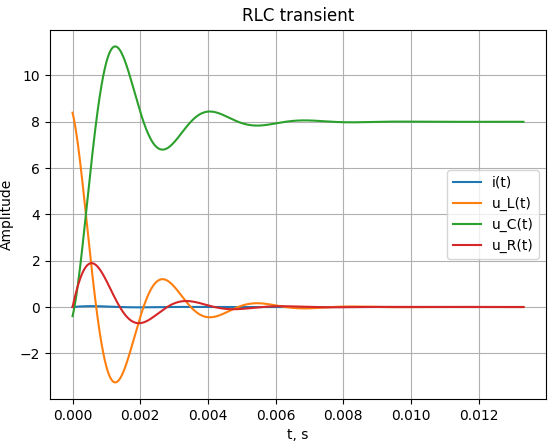
\includegraphics[width=0.5\textwidth]{graph-.png}
        \caption{\centering Графік функцій $i(t)$, $u_L(t)$, $u_C(t)$, $u_R(t)$ при коливальному режимі під час замикання ключа}

    \end{figure}

    Аналітичні вирази для напруг та струму в коливальному режимі RLC-контуру під час розмикання ключа мають вигляд (враховуючи, що $R = R_4$, $L = L_4$, $C = C_4$):

    \[
    i(t) = -\frac{E}{\omega_{\text{в}} L_4}\, e^{-\delta t} \sin(\omega_{\text{в}} t)
    \]

    \[
    u_{L}(t) = E\,\frac{\omega_0}{\omega_{\text{в}}} e^{-\delta t} 
    \sin(\omega_{\text{в}} t - 90^\circ)
    \]

    \[
    u_{C}(t) = E\,\frac{\omega_0}{\omega_{\text{в}}} e^{-\delta t} 
    \sin(\omega_{\text{в}} t + 90^\circ)
    \]

    \[
    u_R(t) = i(t) R_4 = -\frac{ER_4}{\omega_{\text{в}} L_4}\, e^{-\delta t} \sin(\omega_{\text{в}} t)
    \]

    де $\delta = \dfrac{R_4+R_{\text{к}}+R_0}{2L_4}$, а значення $\omega_0$ та $\omega_{\text{в}}$ ті самі.

    Звідси отримаємо:

    \[
    i(t)  = -0{,}059345 e^{-1129{,}2 t} \cdot \sin(2246{,}8 t)
    \]

    \[
    u_L(t) = 8{,}3926 e^{-1129{,}2 t} \cdot \sin(2246{,}8 t + 90^\circ)
    \]

    \[
    u_C(t) = 8{,}3926 e^{-1129{,}2 t} \cdot \sin(2246{,}8 t - 90^\circ)
    \]

    \[
    u_R(t) = -2{,}9672 e^{-1129{,}2 t} \cdot \sin(2246{,}8 t)
    \]

    Побудуємо графік цих 4 функцій:

    \begin{figure}[h!]

        \renewcommand{\thefigure}{\arabic{figure}} % робимо "3.1", "3.2" і т.д.

        \centering
        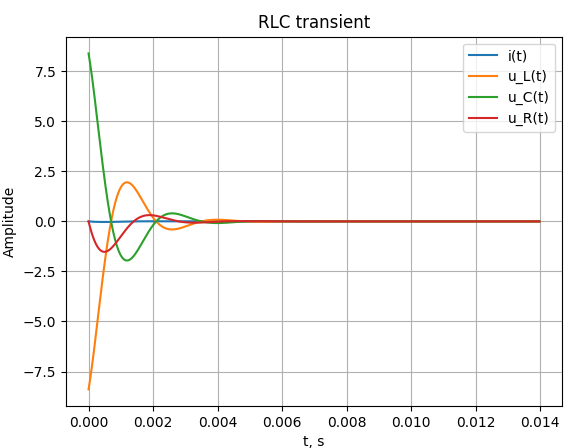
\includegraphics[width=0.5\textwidth]{d.png}
        \caption{\centering Графік функцій $i(t)$, $u_L(t)$, $u_C(t)$, $u_R(t)$ при коливальному режимі під час розмикання ключа}

    \end{figure}

    \noindent
    \textbf{\underline{Висновок:}}
    У ході виконання офлайн частини лабораторної роботи було досліджено перехідні процеси в електричних колах із послідовним з’єднанням RLC-елементів у різних режимах роботи. На основі виміряних параметрів елементів контуру було визначено коефіцієнт загасання, власну частоту та частоту затухаючих коливань. Порівняння аналітичних залежностей із експериментальними осцилограмами показало їхню якісну й кількісну відповідність.

    Було отримано осцилограми напруг $u_R(t)$, $u_L(t)$ та $u_C(t)$ у коливальному режимі та визначено значення опору, за якого система переходить до критичного (аперіодичного) режиму. Експериментально встановлений критичний опір
    \[
    R_{\text{кр/експ.}} \approx 282{,}5\ \Omega
    \]
    майже збігається з теоретичним значенням
    \[
    R_{\text{кр}} \approx 282{,}84\ \Omega,
    \]
    що підтверджує правильність аналітичних розрахунків.

    Також було визначено ємність $C_2$, при якій частота коливань подвоюється. Розрахункове значення 
    \[
    C_2 \approx 0{,}75\ \text{мкФ}
    \]
    узгоджується з експериментальним параметром $C_2 = 0{,}8\ \text{мкФ}$, що свідчить про адекватність теоретичної моделі.

    Окрім експериментальної частини, було виконано аналітичне моделювання перехідних процесів за допомогою мови програмування Python. На основі теоретичних рівнянь були отримані функції для струму та напруг на елементах контуру як у режимі замикання, так і в режимі розмикання ключа. Побудовані графіки відтворюють основні характеристики сигналів: експоненційне загасання амплітуди, фазові зсуви та залежність швидкості згасання від величини активного опору.

    \newpage

    \begin{center} \textbf{\large Завдання №2 (онлайн частина)} \end{center}

    Моя група: ІО-41, і я 6 по списку. Звідси матиму такі параметри:

    \begin{table}[h!]
        \centering
        \begin{tabular}{|c|c|c|c|}
            \hline
            $E$, В & $R$, Ом & $L$, Гн & $C$, мкФ \\
            \hline
            11 & 116 & 0,16 & 9,4\\
            \hline
        \end{tabular}
        \caption{Параметри елементів}
    \end{table}

    \begin{figure}[h!]

        \renewcommand{\thefigure}{\arabic{figure}} % робимо "3.1", "3.2" і т.д.

        \centering
        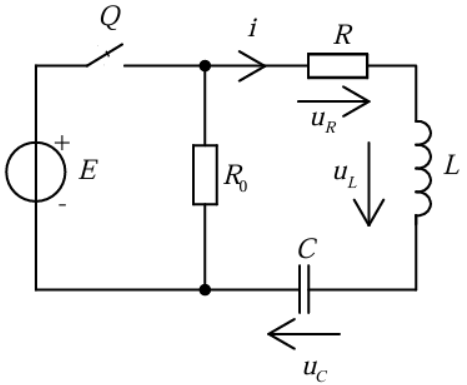
\includegraphics[width=0.4\textwidth]{structure_scheme_online.png}
        \caption{Структурна схема електричного кола}

    \end{figure}

    Загальне характеристичне рівняння кола має вигляд:

    \[
    p^2 + 2\delta p + \omega_0^2 = 0
    \]

    де $\delta = \dfrac{R}{2L}$ (для періодичного режиму), а $\omega_0 = \dfrac{1}{\sqrt{LC}}$

    \vspace{1em}

    Звідси виходить таке характеристичне рівняння:

    \[
    p^2 + 725p + 664893{,}468 = 0
    \]

    \noindent
    Звідси вирішимо це рівняння та зведемо результати обчислювань до однієї таблиці:

    \begin{table}[h!]
        \centering
        \begin{tabular}{|p{6cm}|c|c|c|}
            \hline
            Значення для коренів характеристичного рівняння 
                & $p_1 = -362{,}5 + 730{,}4i$ 
                & $p_2 = -362{,}5 - 730{,}4i$
                & $\tau_1 = \left|\dfrac{1}{\delta}\right|$, мс \\[1.2em]
            \hline
            Характер перехідного процесу:
                & \multicolumn{2}{c|}{Коливальний}
                & 2,76 \\[2.5em]
            \hline
        \end{tabular}
        \caption{Розраховані значення}
    \end{table}

    Тепер обчислимо критичний опір

    \[
    R_{\text{кр}} = 2 \sqrt{\frac{L}{C}} \approx 260{,}93 \text{ Ом}
    \]

    \newpage

    Тепер побудую електричну схему із Рис. 6:

    \begin{figure}[h!]

        \renewcommand{\thefigure}{\arabic{figure}} % робимо "3.1", "3.2" і т.д.

        \centering
        \includegraphics[width=0.5\textwidth]{multisim_scheme.pdf}
        \caption{Схема в Multisim}

    \end{figure}

    Частоту джерела напруги тактової частоти розрахував за умовою, що період коливань є у 10 більший за значення $\tau_1$. Графік напруги на конденсаторі, знятий із осцилографа:

    \begin{figure}[h!]

        \renewcommand{\thefigure}{\arabic{figure}} % робимо "3.1", "3.2" і т.д.

        \centering
        
\includegraphics[width=0.5\textwidth]{graph3.png}
        \caption{Графік періодичних коливань напруги на конденсаторі}

    \end{figure}

    Графік напруги на конденсаторі, знятий із осцилографа при аперіодичному режимі (опір $R = 256$ Ом):

    \begin{figure}[h!]

        \renewcommand{\thefigure}{\arabic{figure}} % робимо "3.1", "3.2" і т.д.

        \centering
        
\includegraphics[width=0.5\textwidth]{graph4.png}
        \caption{Графік аперіодичних коливань напруги на конденсаторі}

    \end{figure}

    Для аперіодичного режиму, $\delta = \dfrac{R + R_0}{2L}$, звідси отримуємо нове характеристичне рівняння, але вже для аперіодичного режиму:

    \[
    p^2 + 1912{,}5p + 664893{,}468 = 0
    \]

    Звідси вирішиимо це рівняння та зведемо результати обчислювань до однієї таблиці:

    \begin{table}[h!]
    \centering
    \begin{tabular}{|p{6cm}|c|c|c|}
        \hline
        $R_{\text{КР}} = 260{,}93$, Ом
            & \multicolumn{2}{c|}{$R_{\text{ап}} = 256$, Ом}
            & $\tau_2 = \left|\dfrac{1}{p_1}\right|$, мс \\[1.2em]
        \hline
        Значення для коренів характеристичного рівняння, при аперіодичному процесі
            & $p_1 = -456{,}73$
            & $p_2 = -1455{,}77$
            & 2,19\\[2.5em]
        \hline
    \end{tabular}
    \caption{Розраховані значення для аперіодичного режиму}
    \end{table}

    \noindent
    На основі усіх розрахованих значень, відновимо аналітичні функції для напруги на конденсаторі $u_C(t)$ (у мене парний варіант) у періодичному та аперіодичному режимах під час замикання ключа.

    Для періодичного режиму:

    \[
    u_{C}(t) = E + E\,\frac{\omega_0}{\omega_{\text{в}}}\, e^{-\delta t}\, \sin(\omega_{\text{в}} t - 90^\circ)
    \]

    Для аперіодичного режиму:

    \[
    u_C(t) = 
    E - \frac{E}{p_2 - p_1}\left( 
        p_2 e^{p_1 t} - p_1 e^{p_2 t}
    \right)
    \]

    де $E = 11$, $\delta = 362,5$ рад/с, $\omega_0 = 815{,}41$ рад/с, $\omega_{\text{в}} = \sqrt{\omega_0^2 - \delta^2} \approx 730{,}40$ рад/с,  $p_1 = $ \\
    $= -456{,}73$ рад/с, $p_2 = -1455{,}77$ рад/с.

    \vspace{1em}

    Тепер побудуємо графіки цих функцій:

    \begin{figure}[h!]

        \renewcommand{\thefigure}{\arabic{figure}} % робимо "3.1", "3.2" і т.д.

        \centering
        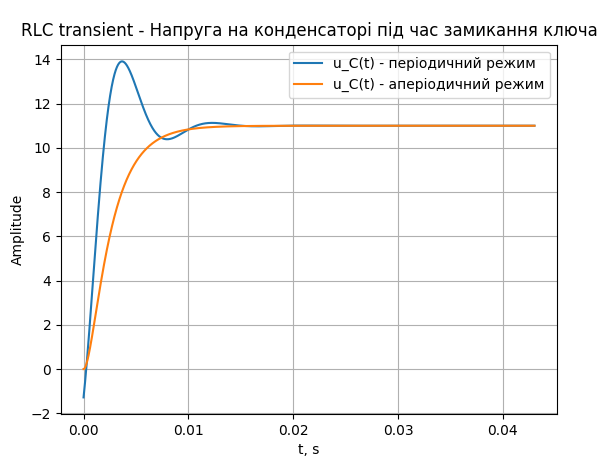
\includegraphics[width=0.5\textwidth]{fin.png}
        \caption{\centering Графіки функцій $u_C(t)$ у періодичному та аперіодичному режимах під час замикання ключа}

    \end{figure}

    \newpage

    \noindent
    \textbf{\underline{Висновок:}} У періодичному режимі (при $R < R_{\text{кр}}$) напруга на конденсаторі має коливальний характер із затухаючими коливаннями навколо усталеного значення $U_C \approx E$. Спостерігається перевищення напруги над ЕРС джерела (перерегулювання) та поступове зменшення амплітуди коливань зі сталою часу $\tau_1 \approx 2{,}76$ мс. Це відповідає комплексно-спряженим кореням характеристичного рівняння й підтверджує коливальний характер процесу.

В аперіодичному режимі (при $R$, близькому до $R_{\text{кр}}$ та вибраному $R_{\text{ап}} = 256$ Ом) напруга на конденсаторі зростає монотонно, без коливань та перерегулювання, що відповідає дійсним від'ємним кореням характеристичного рівняння $p_1$ та $p_2$. Час встановлення напруги визначається сталою часу $\tau_2 \approx 2{,}19$ мс і є меншим, ніж час затухання у періодичному режимі, тобто система швидше входить в усталений стан без коливань.

Отже, чисельне моделювання та аналітичні розрахунки показали, що зміна активного опору $R$ дозволяє керувати характером перехідного процесу: при $R < R_{\text{кр}}$ коло має коливальний (затухаючий) режим, а при $R \approx R_{\text{кр}}$ — аперіодичний, із монотонним наближенням напруги на конденсаторі до усталеного значення. Отримані результати підтверджують теоретичні положення про вплив параметрів RLC-кола на перехідні процеси.

\end{document}